\subsection{Scenario-Aware Synthetic Data Generation}
\label{sec:method_generation}

\subsubsection{StoryConfig and Scenario Specification}

Synthetic tenant generation begins with a \texttt{StoryConfig} that defines the company profile and the narrative arc the generator must realize. The configuration includes the company name, industry, company size, number of users, duration of the simulation, and a list of key events that anchor the narrative. This representation is compact enough for rapid scenario design yet expressive enough to vary organizational complexity and event density. The same generator can therefore instantiate a university administration scenario, a legal-services scenario, or a software-incident scenario without changing the code path.

\begin{table}[t]
\centering
\caption{Core fields in the \texttt{StoryConfig} specification.}
\label{tab:storyconfig_fields}
\small
\begin{tabular}{p{0.22\linewidth}p{0.14\linewidth}p{0.52\linewidth}}
\toprule
\textbf{Field} & \textbf{Type} & \textbf{Purpose} \\
\midrule
\texttt{company\_name} & string & Names the tenant and appears in prompts and output paths \\
\texttt{industry} & string & Conditions vocabulary, artifacts, and domain-specific events \\
\texttt{company\_size} & string & Influences organizational breadth and communication patterns \\
\texttt{num\_users} & int & Sets the size of the user roster and social graph \\
\texttt{duration\_days} & int & Controls the temporal window over which history accumulates \\
\texttt{key\_events} & list[string] & Defines narrative milestones that should recur across modalities \\
\texttt{description} & string & Supplies free-form scenario context to the generator prompts \\
\bottomrule
\end{tabular}

\end{table}

\subsubsection{Five-Stage Generation Pipeline}

The generator executes in five stages. It first creates the directory scaffold and initializes modality-specific YAML files. It then generates the user roster in batches, using diversity prompts to avoid name collisions and departmental imbalance. Next, it iterates day by day through the simulation, producing 3--5 narrative events per day while maintaining rolling history buffers. It materializes those events as emails, chats, meetings, and files, and it finally writes a complete \texttt{generation\_log.json} that serves as the source material for evaluation-case generation. The pipeline is incremental by design: artifacts are appended to disk as they are generated, which supports large tenants without requiring all content to remain in memory.

\begin{table}[h]
\centering
\caption{Five-stage tenant-generation process.}
\label{tab:generation_pipeline}
\small
\begin{tabular}{p{0.07\linewidth}p{0.22\linewidth}p{0.60\linewidth}}
\toprule
\textbf{Stage} & \textbf{Name} & \textbf{Output and purpose} \\
\midrule
1 & Directory scaffold and initialization & Creates tenant directories, empty modality YAML files, and a persistent workspace for generated documents \\
2 & User generation with diversity control & Produces the employee roster, titles, departments, managers, skills, and group memberships while avoiding duplicates \\
3 & Daily narrative generation & Expands key events into day-level story beats using recent-history and long-history buffers to preserve temporal coherence \\
4 & Artifact materialization and cross-referencing & Generates emails, chats, meetings, and files whose content explicitly references shared events and decisions \\
5 & Evaluation-log export & Serializes the full event history into \texttt{generation\_log.json} for downstream query generation and auditability \\
\bottomrule
\end{tabular}

\end{table}

\subsubsection{Content Type Generation}

Each artifact type is generated with a schema tailored to its role in enterprise communication. Emails are produced in two steps: a summary pass proposes sender, recipients, subject, and context, and a second pass expands that summary into realistic prose. Chats are likewise generated from conversation summaries into timestamped message sequences. Meetings produce three linked artifacts: metadata, transcript, and sidebar chat. Files are created as both metadata entries and concrete documents inside the sandboxed file tree. This staged process gives the generator enough structure to maintain consistency while still allowing varied surface realizations.

\subsubsection{Narrative Coherence Mechanisms}

Long-range coherence is preserved through explicit memory structures rather than through prompt length alone. A recent-history buffer stores the last several days of events verbatim, while a long-history buffer stores compressed summaries of earlier periods. Every seven simulated days, the recent buffer is summarized and appended to the long-term history. This mechanism allows later generations to mention prior incidents, decisions, and unresolved tensions without forcing the model to ingest the entire raw history each day. Cross-document references are then encouraged directly in the prompts, so that an email can cite a meeting outcome, a file can summarize a discussion from chat, and a report can reference both.

\begin{figure}[h]
\centering
%\fbox{\parbox{0.96\linewidth}{%
%\vspace{4pt}
%\small\color{blue}\itshape\raggedright
%\textbf{[Figure placeholder --- generation pending.]}
%A directed graph illustrating synthetic artifact creation and inter-document linkage within a single generated tenant.
%\textbf{Top-center node:} A dark-blue rounded rectangle labeled ``StoryConfig'' with five child annotation labels fanning out: company name, industry, num\_users, duration\_days, key\_events.
%\textbf{Below StoryConfig:} A horizontal five-stage chevron pipeline strip (Stage~1:~Directory Scaffold $\rightarrow$ Stage~2:~User Generation $\rightarrow$ Stage~3:~Daily Narrative $\rightarrow$ Stage~4:~Artifact Materialization $\rightarrow$ Stage~5:~Log Export), styled with left-pointing chevron shapes in mid-blue tones. A downward arrow from StoryConfig enters Stage~1.
%\textbf{Below the pipeline strip:} Four vertical artifact ``lanes'' separated by thin gray dividers (left to right):
%\textit{Lane~1 (Emails, blue-teal)}: A stack of four envelope icons at timestamps Day~1, Day~3, Day~7, Day\ldots, connected by thin timeline arrows.
%\textit{Lane~2 (Meetings, teal)}: Calendar+speech-bubble icons at Day~2, Day~5, Day~9.
%\textit{Lane~3 (Files, teal-green)}: Document icons at Day~4, Day~8.
%\textit{Lane~4 (Chats, green)}: Speech-bubble chain icons at Day~1, Day~3, Day~6, Day~10.
%\textbf{Cross-lane dashed red arrows} showing inter-artifact references (labeled):
%``references person'' (Email Day~3 $\rightarrow$ User node);
%``cites file'' (Meeting Day~5 $\rightarrow$ File Day~4);
%``follows up on meeting'' (Chat Day~6 $\rightarrow$ Meeting Day~5);
%``triggered by email'' (File Day~8 $\leftarrow$ Email Day~7).
%These cross-lane arrows represent the dependency links that enable multi-hop reasoning queries.
%\textbf{Bottom:} A horizontal shared timeline bar spanning all four lanes, labeled ``Simulated timeline (Day~1 \ldots Day~$N$)'' with evenly spaced tick marks.
%Below the timeline, two overlapping buffer icons: ``Recent-history buffer (last $k$ days verbatim)'' and ``Long-history buffer (compressed summaries)'' connected by a ``summarize every 7 days'' arrow.
%Color scheme: StoryConfig box and pipeline chevrons in deep blue; lane icons in teal-to-green gradient; cross-lane arrows in crimson; timeline bar in medium gray; buffer icons in light blue.
%\vspace{4pt}
%}}
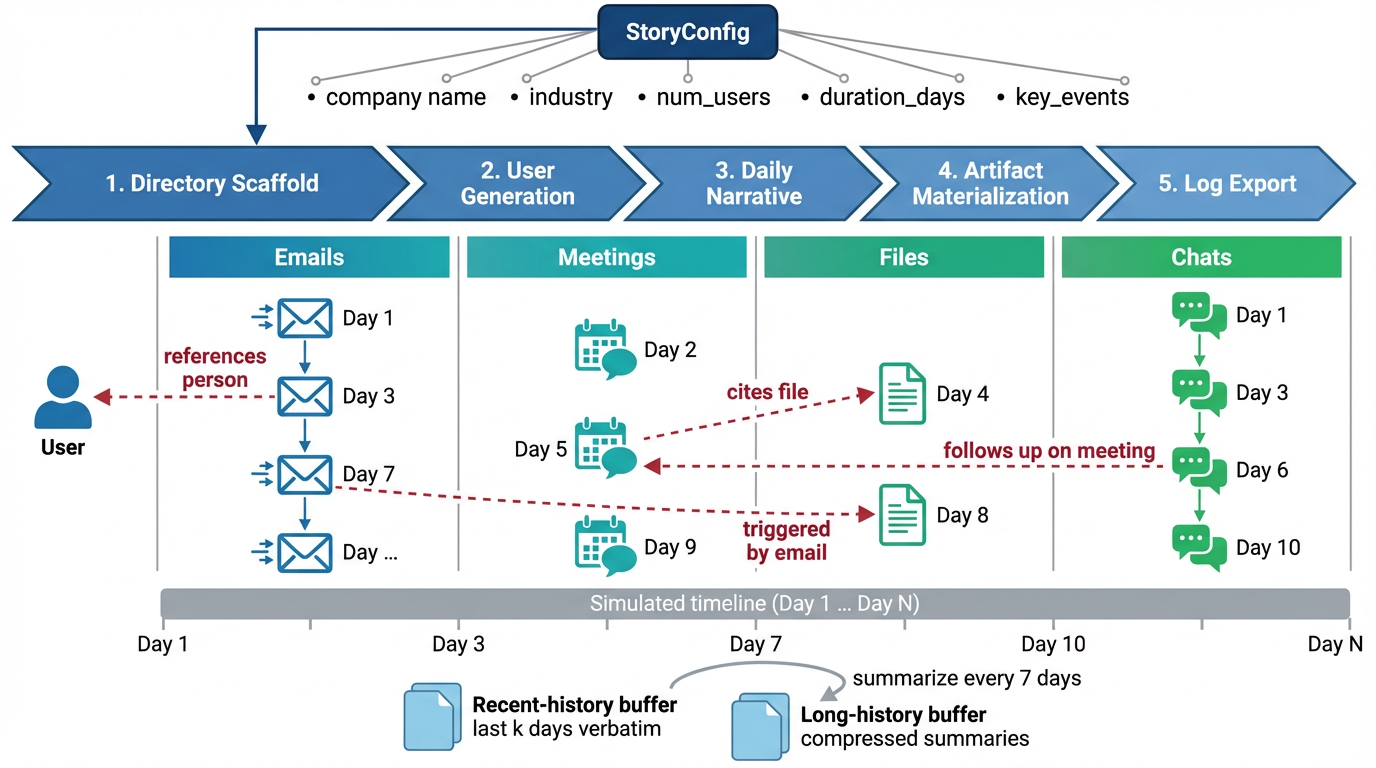
\includegraphics[width=0.9\textwidth]{figures/tenant-generation-pipeline.png}
\caption{EABench five-stage tenant-generation pipeline and inter-artifact linkage graph. A single \texttt{StoryConfig} drives the parallel creation of emails, meetings, files, and chats, which are connected by explicit cross-document references along a shared temporal timeline. These cross-references are what enable multi-hop and temporal reasoning evaluation cases.}
\label{fig:data_generation}
\end{figure}